\iffalse

Nico Casale
Cody Orazymbetov

ECE 592 Project 2

\fi

\documentclass[]{../ncmathy}

\begin{document}

After implementing the A* algorithm and verifying that it yields the same result as Dijkstra's algorithm, we ran the same experiment as before with some modifications. Being that the A* algorithm requires a pre-calculated heuristic function, we used the same destination and calculated a random assortment of distances to the destination. The heuristic function depends only on the destination, so we saved some simulation time by considering only a variety of paths to the same destination. The heuristic function is used by the A* algorithm to guide the iterations toward the goal in an optimal manner. When considering nodes, the heuristic function gives an estimate for the distance from a given node to the goal node (destination.) This, ideally, should allow the algorithm to find the best path more quickly. We found that our algorithm didn't perform very well, but has potential to. Firstly, it's not really faster than our Dijkstra implementation. The Wikipedia article for the A* algorithm indicates that the heuristic function is the main factor that determines the order of complexity. If the search tree is not organized in an effective manner, the algorithm's runtime suffers. The heuristic function generates an implicit search tree based on its biases, and the article mentions that the optimal heuristic function is monotonic and admissible. 
\\\\
As we expect, keeping track of the heuristic data requires $|V|$ extra memory locations to store the distance of each node to the destination. MATLAB uses double-precision, but lower-precisions could be tried, as the heuristic function is meant mainly to point in the general direction. In addition, the pre-calculation is $O(|V|^2)$ as we are using Dijkstra's Algorithm to obtain the heuristic function. 
\\\\
The figure below shows the results of our experiment over many cities with final destinations of Raleigh and Charlotte. 5000 distances were found to each destination. Note that the runtime appears linear in the number of nodes traversed. However, the linear regression is skewed, because it's sensitive to the outliers. We also expect that the higher run-time of our implementation of the A* algorithm is due to a na\"ive coding scheme that doesn't maximize processing efficiency.

\begin{figure}[H]
\centering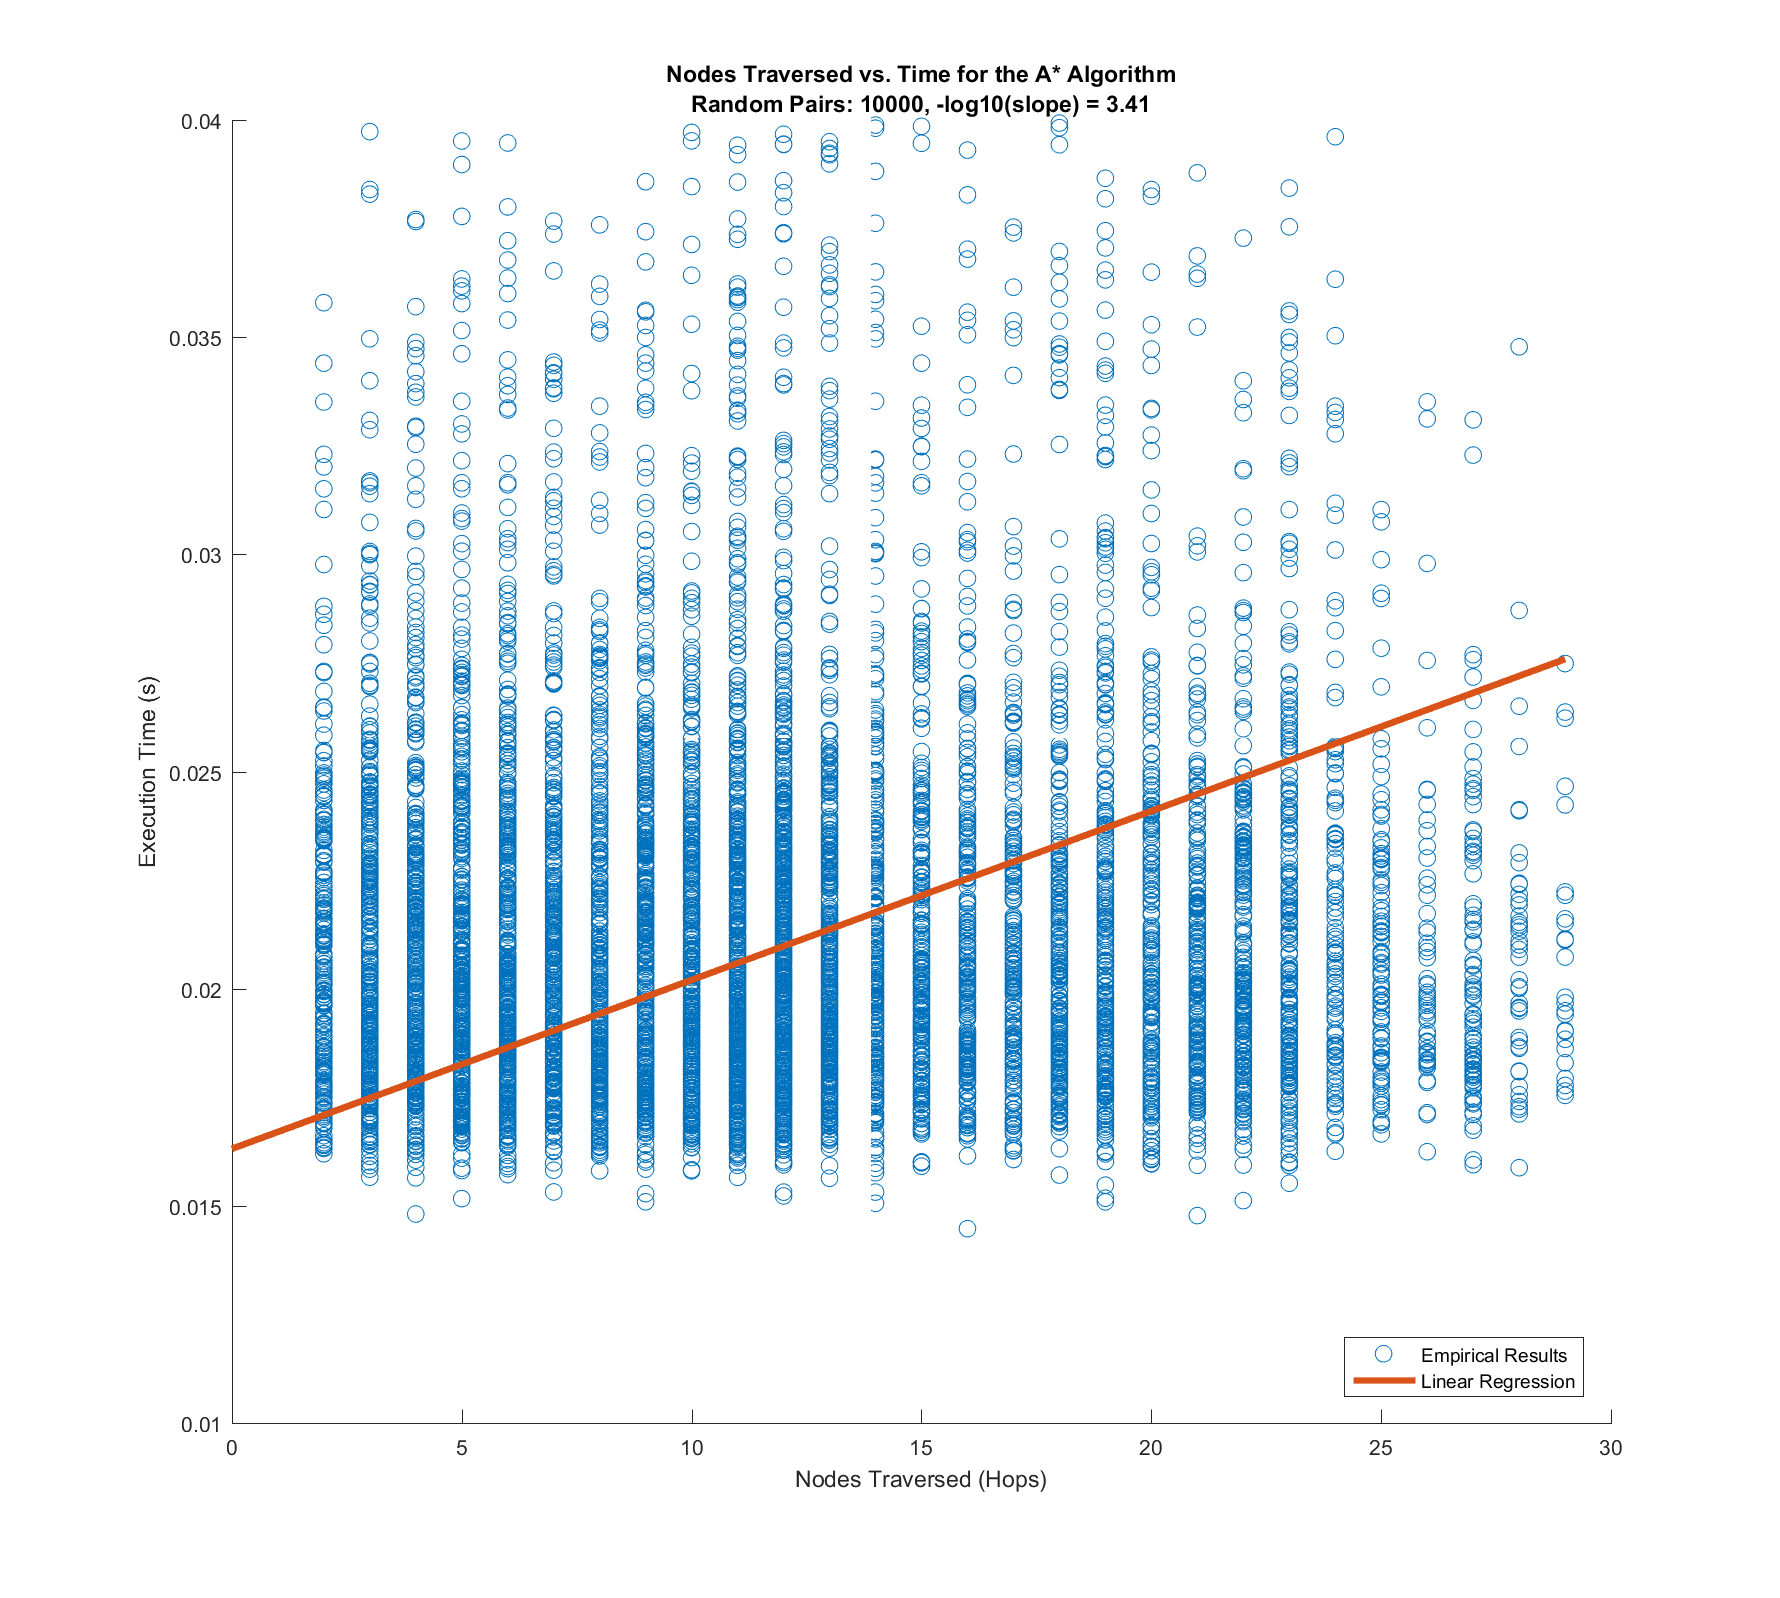
\includegraphics[width=0.8\textwidth]{AstarEmpirical}
\caption{Empirical results of the A* Algorithm.}
\end{figure}

\end{document}